%! Licence = CC BY-NC-SA 4.0

%! Author = gianfluetsch
%! Date = 22. Jan 2022
%! Project = icth_summary

\section{Verschlüsselung}
\subsubsection{A}
Mit RSA-verschlüsselte Nachricht c=8 abgefangen und kennen öffentlichen Schlüssel des Empfängers (e=13, n=323).
Aus sicherer Quelle wissen Sie, dass eine der beiden Primzahlen 17 ist. Entschlüsseln Sie die Nachricht!\\
Gegeben: $c=8, e=13, n=323, p=17$\\
$solve(323=17*x,x) \rightarrow q=19$\\
$\phi(n) = (p-1)*(q-1) = 16*18=288$\\
$d=\frac{2*\phi(n)+1}{e}=\frac{2*288+1}{13}$\\
$d=rsa\_ereuk(17,288) \rightarrow d=17$\\
$rsa\_dec(8,13,323) \rightarrow m=179$\\
$\rightarrow$ d negativ $\rightarrow$ d=Wert in obiger Spalte nehmen

\subsubsection{B}
Mit RSA-verschlüsselte Nachricht c=4 abgefangen und kennen öffentlichen Schlüssel des Empfängers (e=13, n=143).
Beide Primzahlen (p \& q) sind grösser als 10. Entschlüsseln Sie die Nachricht!\\
Gegeben: $c=8, e=13, n=143$\\
$p=11, q=13 \rightarrow 11*13 = 143$\\
$\phi(n) = (p-1)*(q-1) = 10*12=120$\\
$d=\frac{2*\phi(n)+1}{e}=\frac{2*288+1}{13}$\\
$d=rsa\_ereuk(13,120) \rightarrow d=37$\\
$rsa\_dec(4,13,143) \rightarrow m=108$

\subsubsection{C}
Es wird ein asymmetrisches Verfahren (RSA) verwendet. Wie viele verschiedene Schlüsselpaare müssen erzeugt werden, wenn in einer Gruppe von 25 Teilnehmern. jeder mit jedem vertraulich kommunizieren möchte?\\
\textit{25 Schlüsselpaare}\\

Wie viele Schlüssel muss jeder Teilnehmer speichern, wenn sie davon ausgehen, dass es eine vertrauenswürdige „Schlüsselbank“ gibt, bei der die öffentlichen Schlüssel abgefragt werden können?\\
\textit{Bei einer öffentlichen Schlüsselbank. Nur seinen Private Key (und ggf. noch seinen öffentlichen).}\\

Teilnehmer a möchte an Teilnehmer b eine verschlüsselte und signierte Nachricht versenden. Welche Schlüssel verwendet
\begin{itemize}
    \item User a: \textit{public Key von b und private Key von a}
    \item User b: \textit{public Key von a und private Key von b}\\
\end{itemize}

Kommt es bei der Anwendung durch die Teilnehmer a und b dabei auf die Reihenfolge der Schlüssel an?\\
\textit{Nein}\\

\paragraph{Gegeben seien die beiden Primzahlen 11 und 5}\mbox{}\\
Bestimmen sie die Zahl \textit{n} und die Zahl $\phi(n)$\\
$n=11*5=55$\\
$\phi(n) = 10*4=40$

\paragraph{Zur Verschlüsselung wird der öffentliche Schlüssel e  = 17 verwendet}\mbox{}\\
Ermitteln sie den privaten Schlüssel d zum Entschlüsseln einer Nachricht.\\
Es muss gehlten: $e*dmod\phi(n)=1$\\

\begin{center}
    \vspace{-8pt}
    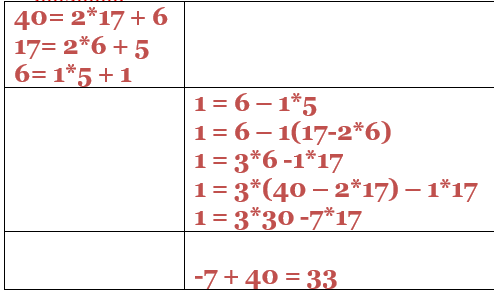
\includegraphics[width=.7\linewidth]{./01-quellencodierung/fs2017_4}
    \vspace{-8pt}
\end{center}

$rsa\_euklid(17,40)$\\

Daraus folgt, 33 ist die Inverse zu 17 bzgl. der mod40 Rechnung. D.h. der Schlüssel zum Entschlüsseln ist 33.

\subsubsection{D}
91 Teilnehmer wollen paarweise vertraulich Informationen austauschen.\\

In einem ersten Ansatz wird ein symmetrisches Verfahren gewählt. 
Wie viele verschiedene Schlüssel müssen erzeugt werden, wenn jeder mit jedem vertraulich kommunizieren möchte?\\
$91/2*90=4095$ oder $nCr(91,2)=4096$\\

Wie viele Schlüssel muss jeder Teilnehmer speichern?\\
\textit{N=90}\\

\subsubsection{E}
Handel es sich bei der Cesar-Verschlüsselung um ein symmetrisches oder asym-metrisches Verfahren?\\
\textit{Um ein symmetrisches Verfahren}\\

Wird bei diesem Verfahren jedes Quellzeichen einzeln Verschlüsselt oder werden immer mehrere Quellzeichen zur Verschlüsselung zusammengefasst?\\
\textit{Es wird jedes Quellzeichen einzeln codiert}\\

Beschreiben Sie, wie sie in diesem Fall eine einfache Kryptoanalyse machen können und was sie dazu brauchen?\\
\textit{Bei einer Cesar-Verschlüsselung werden die Häufigkeiten der Quellzeichen nicht verwürfelt. Ist die Zielsprache bekannt ist auch das häufigste Zeichen der Spra-che bekannt. Ist der Erhaltene Code gross genug kann mit einer einfachen Häu-figkeitsanalyse der Schlüssel ermittelt werden.}\\

\columnbreak

Gegeben seien die beiden Primzahlen 15 und 11. Als öffentlichen Schlüssel wählen Sie die Primzahl 17.\\
Berechnen sie den inversen, privaten Schlüssel und machen sie alle Zwischenschritte deutlich.\\
$n = 143 \rightarrow \phi(n)=12*10=120$\\
Es muss gelten: $e*d mod \phi(n) = 1$\\
$120=17*7+1$\\
$7=1*7+0$\\

$1=120-17*7$\\
$1=-17*7mod120 + 120 * 7$\\
$1=103*7mod120$\\
$7^{-1}mod120=113$\\

$rsa\_euklid(17,120) \rightarrow d=113$\\

Daraus folgt, 113 ist der Inverse Schlüssel.\\

Verschlüsseln Sie die Zahl 3 mit dem öffentlichen Schlüssel 17, mache sie die Rechenschritte deutlich.\\
$=3^{17}mod143$\\
$=3^{10}*3^7mod143$\\
$=9$\\

$rsa\_enc(3,17,143) \rightarrow 9$\\

Welchen Schlüssel verwenden sie, um eine Nachricht zu:\\
\begin{itemize}
    \item Unterschreiben: \textit{eigenen private Key}
    \item Verschlüsseln: \textit{public Key vom Empfänger}
\end{itemize}